\documentclass{article}

% Pakete
\usepackage[utf8]{inputenc}
\usepackage[ngerman]{babel}
\usepackage{amsmath}
\usepackage{graphicx}
\usepackage{float}
\usepackage{cite}
\usepackage{multirow}
\usepackage{booktabs}
\usepackage{url}
\usepackage{geometry}
\usepackage{hyperref}
\usepackage{fancyhdr}
\usepackage{setspace}
\usepackage{caption}
\geometry{
    left=0.25in,
    right=0.25in,
    top=0.25in,
    bottom=0.25in
}


% Titel und Autor
\title{RNA Analytik}
\author{Thorsten Enge \and David Maruhn}
\date{\today}

\begin{document}

% Titel erstellen
\maketitle

% Inhaltsverzeichnis
\tableofcontents
\newpage

% Einleitung
\section{Einleitung}

Während bei der DNA-Analytik untersucht wird, ob eine bestimmte DNA-Sequenz auf dem Genom vorhanden ist, wird bei der RNA-Analytik untersucht, ob und wie stark ein bestimmtes Gen transkribiert wird. Das Vorhandensein eines Gens auf dem Genom bedeutet nicht zwangsläufig, dass dieses Gen auch transkribiert wird. Mechanismen wie die DNA-Methylierung, die Histonmodifikation, Transkriptionsfaktoren und Enhancer bzw. Silencer beeinflussen die Transkription eines Gens. Die durch die Analyse der RNA kann einerseits das Vorhandensein eines Gens auf dem Genom bestätigt werden, andererseits kann durch die quantifizierung Rückschlüsse auf die Transkriptionsrate gezogen werden und somit auf die Aktivität des Gens. Das nichtvorhandensein eines Transkripts bedeutet entweder das Fehlen des Gens auf dem Genom oder eine sehr geringe Transkriptionsrate. 

% Materialien und Methoden
\section{Materialien und Methoden}

\subsection*{Zellkulturen}
Für die RNA-Isolation wurden die Zelllinien HEK293T und A375 verwendet.
Beide Zellkulturen sind immortale humane Zelllinien.
\begin{itemize}
    \item HEK293T sind Zellen, die aus der Niere eines Embryos gewonnen wurden.
    Sie sind durch die Transformation mit dem SV40-T-Antigen immortalisiert
    worden.
    \item A375-Zellen stammen aus einem Melanom, sind sie von natur aus
    immortalisiert.
\end{itemize}

\subsection*{Genes of Interest}
Die Gene of Interest sind die Gene, die in dieser Arbeit quantifiziert
werden sollen. In diesem Fall sind es die Gene GAPDH und Beta-Actin.
\begin{itemize}
    \item GAPDH (Glyceraldehyde-3-phosphate dehydrogenase) katalysiert die 
    Oxidation von Glyceraldehyd-3-phosphat zu
    1,3-Bisphosphoglycerat im Glykolyseweg.
\[
\text{C}_3\text{H}_5\text{O}_6\text{P} + \text{NAD}^+ + \text{P}_i \xrightarrow{\text{GAPDH}} \text{C}_3\text{H}_4\text{O}_{10}\text{P}_2 + \text{NADH} + \text{H}^+
\]

    \item Beta-Actin wird in der qPCR als Referenzgen verwendet, da es in allen
    Zellen in gleicher Menge vorhanden ist und somit als Kontrollgen dient.
    
\end{itemize}


\section{Durchführung}

Die RNA wird aus zwei unterschidllichen Zelllinien isoliert und anschließend mittels einer reverse Transkription in cDNA transkribiert. Die cDNA wird dann mittels qPCR quantifiziert.

\subsection{RNA-Isolation mittels Monarch\textsuperscript{\textregistered} Total RNA Miniprep Kit (NEB)}

\begin{enumerate}
    \item Lysat erstellen
    \item gDNA entfernen
    \item RNA isolieren und Nebenprodukte entfernen, unter Nutzung
    von Ethanolpräzipitation, um die Haftung der RNA zu erleichtern.
    \item DNase 1 zerstört Reste der DNA
    \item Elution RNA in nukleasefreiem Wasser
\end{enumerate}

\subsubsection*{RNA-Isolation}
In diesem Versuch wurde die RNA aus kultivierten
humanen Zellen isoliert. Zu beachten sind die
sorgfältige Reinigung von allen Oberflächen und Geräten
mit 70\,\%{}igem Alkohol, um Verunreinigungen mit
Nukleasen zu vermeiden. Aus gleichem Grund ist es sinnvoll,
stets mit Handschuhen zu arbeiten.
Dafür wurden zunächst die tiefgefrorenen Zellpellets der
kultivierten Zellen aufgetaut, bei 4 °C für 2 Minuten bei
10.000 rpm zentrifugiert und durch Zugabe von 800 µl des
Lysepuffers in Lysat überführt. 
Durch die Lyse werden die Zellen aufgebrochen
und der Zellinhalt für die weitere Prozessierung zugänglich gemacht.
Im nächsten Schritt wurde aus dem Lysat die gDNA, die genomic DNA,
durch Waschung über einer Removal Column entfernt.
Hierfür wurden 800 µl Lysat in das gDNA Removal Column
überführt und für 1 Minute bei 10.000 rpm und
Raumtemperatur (RT) zentrifugiert.
Die Column macht sich die strukturellen Unterschiede der
DNA und RNA zunutze, um die DNA zu fixieren. Der flüssige
Durchsatz wurde nach Entfernen und Entsorgung der gDNA Removal
Column im Verhältnis 1:1 mit Ethanol (\(\geq\) 95\%) gemischt.
Die Mischung wurde in mehreren Durchgängen in die RNA Purification
Column überführt und für 1 Minute, 10.000 rpm und RT zentrifugiert.
Der Durchsatz wurde nach jedem Durchgang verworfen. Der Prozess
wurde wiederholt, bis die Mischung einmal komplett durch die RNA Removal
Column zentrifugiert wurde. 
Anschließend wurde die RNA Removal Column mit 500 µl RNA Wash Buffer
benetzt und nochmals für 1 Minute zentrifugiert. Der Durchsatz wurde verworfen.
Im nächsten Schritt wurde die RNA Removal Column in ein Tube
überführt, das 75 µl DNAse I Reaction Buffer enthält und die Matrix
mit DNAse I benetzt. 
Das Tube wurde 15 Minuten bei RT inkubiert. Danach wurden 500 µl Wash
Buffer auf die Säule pipettiert, 1 Minute zentrifugiert und der
Überstand verworfen. Anschließend wurden 500 µl Priming Buffer auf die
Säule pipettiert, 1 Minute zentrifugiert und der Überstand verworfen.
Es folgte eine Waschung mit 500 µl Wash Buffer und 1 Minute Zentrifugation.
Nach Verwerfen des Überstands wurde nochmals mit 500 µl Wash Buffer auf die
Säule pipettiert, 2 Minuten zentrifugiert und der Überstand entfernt.
Die Säule wurde in ein nukleasefreies Tube überführt.
Es folgte die Elution der RNA, indem 50 µl nukleasefreies
H$_2$O auf die Matrix der Säule pipettiert und 1 Minute zentrifugiert wurde.
Die genaue Vorgehensweise ist der Anleitung des Monarch
Total RNA Miniprep Kit (NEB) zu entnehmen.

\subsubsection*{Spektroskopie zur Bestimmung der Nukleinsäurenkonzentration}

Dieser Abschnitt findet statt, um die Qualität der
Aufbereitung der RNA aus den Zellpellets zu bewerten.
Hierfür wurde 1µl der Probe vermessen. Ziel war es,
das Verhältnis der Absorption der Wellenlänge 260/280 [nm] zu überprüfen.
Der experimentelle Schwellwert für eine weiterverwendbare RNA-Konzentration
in der Probe ist ca. 2,0. Die Messung fand in einem Spektrophotometer
\mbox{DS-11+ -DeNovix} statt. Benutzt wurde das RNA-Programm.
Zunächst wird eine blank-messung durchgeführt,
um dem Spektrophotometer einen Bezugsrahmen für folgende Messungen zu geben.
Dies erfolgt durch die Messung 1 µl nukleasefreies H$_2$O. Die Messung
erfolgte über die Mikrovolumenabsorptionseinheit. Nach der Eichung des
Referenzrahmens folgte die Messung der einzelnen Proben. Stets mit 1 µl
Probe auf der Mikrovolumenabsorptionseinheit, die nach jeder Messung mit
nukleasefreiem H$_2$O gereinigt wurde.
    

\subsection{cDNA-Synthese aus isolierter RNA}

\begin{itemize}
    \item Mischen der Komponenten in spezifischer Reihenfolge
    \item Inkubation
\end{itemize}

\subsubsection*{Reverse Transkription - cDNA-Synthese aus isolierter RNA}

Zunächst wurde ein Heizblock TS pro - CellMedia auf 25 °C,
5 Minuten und nicht schüttelnd voreingestellt. Der Puffer,
dNTPs, Random Primer Mix und RNA wurden auf Eis aufgetaut.
RNAse Inhibitor und M-MuLV Reverse Transkriptase wurden bei -20 °C gelagert.
Für die RT-PCR wurde ein Reaktionsvolumen von 20 µl festgelegt.

\begin{table}[H]
\centering
\begin{tabular}{|l|l|}
\hline
\textbf{Komponenten} & \textbf{Volumen} \\ \hline
Random Primer Mix & 2 µl \\ \hline
10X M-MuLV RT Puffer & 2 µl \\ \hline
10 mM dNTP & 1 µl \\ \hline
RNAse Inhibitor (40 U/µl) & 0.2 µl \\ \hline
M-MuLV Reverse Transkriptase (200 U/µl) & 1 µl \\ \hline
RNA (5 µg) & Probenabhängige Konzentration \\ \hline
Nukleasefreies H\textsubscript{2}O & Bis 20 µl auffüllen \\ \hline
\end{tabular}
\caption{Komponenten für die cDNA-Synthese}
\end{table}

Die angegebenen Komponenten wurden in ein 1,5 ml
Eppendorf-Gefäß gefüllt und abzentrifugiert.
Abschließend wurde die Inkubation im Heizblock vorgenommen.
Diese erfolgte in drei Schritten:

\begin{table}[H]
    \centering
    \begin{tabular}{|c|c|}
    \hline
    \textbf{Zeit} & \textbf{Temperatur} \\ \hline
    5 Minuten & 25 °C \\ \hline
    60 Minuten & 42 °C \\ \hline
    20 Minuten & 65 °C \\ \hline
    \end{tabular}
    \caption{Inkubationszeiten und Temperaturen}
    \end{table}

\subsection{Quantifizierung durch qPCR (Real-Time PCR)}

\begin{itemize}
    \item 3 Mastermixe erstellen (je Primer-Paar)
    \item PCR im Cycler
\end{itemize}

\subsubsection*{Quantifizierung durch qPCR}
Zur Untersuchung von drei Primern wurde jeweils ein
Master Mix mit 80 µl Reaktionsvolumen für eine Messung,
eine Zweitmessung und eine NTC in 20 µl vorbereitet.
Jeder Master Mix enthielt pro Reaktion (20 µl) 10 µl 2X Biozym HRM Mix,
0.4 µl 10 µM Primer forward, 0.4 µl 10 µM Primer reverse, 8.2 µl
nukleasefreies H\textsubscript{2}O und 1 µl cDNA oder
nukleasefreies H\textsubscript{2}O für die NTC. Die Master Mixe
wurden in PCR-Tubes transferiert. Die cDNA und das
alternative H\textsubscript{2}O wurden als letztes pipettiert.
Anschließend wurden die PCR-Tubes verschlossen und auf Eis gelegt.
Die Proben wurden in einem Roche Light Cycler 96 mit folgendem
Programm analysiert:

\begin{table}[H]
    \centering
    \begin{tabular}{|l|l|l|l|}
    \hline
    \textbf{Cycles} & \textbf{Step} & \textbf{Temp [°C]} & \textbf{Time [sec]} \\ \hline
    1 & Preincubation & 95 & 120 \\ \hline
    \multirow{2}{*}{40} & \multirow{2}{*}{2 Step Amplification} & 95 & 5 \\ \cline{3-4}
     &  & 65 & 30 \\ \hline
    \multirow{4}{*}{1} & \multirow{4}{*}{High Resolution Melting} & 95 & 60 \\ \cline{3-4}
     &  & 40 & 60 \\ \cline{3-4}
     &  & 65 & 1 \\ \cline{3-4}
     &  & 97 & 1 \\ \hline
    1 & Cooling & 37 & 30 \\ \hline
    \end{tabular}
    \caption{PCR-Zyklusprogramm}
    \end{table}
  

    Natürlich, hier ist der überarbeitete Abschnitt:

\subsection{Analyse der Zielgene}
Um die qPCR-Ergebnisse korrekt interpretieren zu können, wurden zunächst die Transkriptvarianten für GAPDH und Beta-Actin im RefSeq der NCBI-Datenbank identifiziert. Anschließend wurden die Primersequenzen mit den Sequenzen der verschiedenen Transkriptvarianten verglichen, um potenzielle Unterschiede in der Affinität der Primer zu den verschiedenen Transkripten zu ermitteln. Diese Analyse wurde mithilfe eines Python-Skripts durchgeführt.
    
\section{Ergebnisse}

\subsection*{Analyse der Zielgene}


\begin{table}[ht]
    \centering
    \begin{tabular}{|l|l|c|c|c|}
    \hline
    \textbf{Gen} & \textbf{Transkriptvariante} & \textbf{mRNA} & \textbf{Amplifikat ohne Primer} & \textbf{Amplifikat} \\ \hline
    \multirow{6}{*}{GAPDH\_1} & Variant 7 & 1231 & 113 & 154 \\ \cline{2-5} 
                              & Variant 2 & 1386 & \multicolumn{2}{c|}{Forward Primer nicht in Sequenz} \\ \cline{2-5} 
                              & Variant 3 & 1377 & 167 & 208 \\ \cline{2-5} 
                              & Variant 4 & 1525 & 167 & 208 \\ \cline{2-5} 
                              & Variant 1 & 1285 & 167 & 208 \\ \cline{2-5} 
                              & Variant 6 (non-coding) & 763 & 167 & 208 \\ \hline
    \multirow{6}{*}{GAPDH\_2} & Variant 7 & 1231 & 221 & 269 \\ \cline{2-5} 
                              & Variant 2 & 1386 & 221 & 269 \\ \cline{2-5} 
                              & Variant 3 & 1377 & 221 & 269 \\ \cline{2-5} 
                              & Variant 4 & 1525 & 221 & 269 \\ \cline{2-5} 
                              & Variant 1 & 1285 & 221 & 269 \\ \cline{2-5} 
                              & Variant 6 (non-coding) & 763 & \multicolumn{2}{c|}{Forward und Reverse Primer nicht in Sequenz} \\ \hline
    Beta-Actin               &  & 1812 & 339 & 385 \\ \hline
    \end{tabular}
    \caption{Länge der Amplifikate in Basenpaaren (bp): 3. Spalte länge der mRNA, 4. Spalte länge des Amplifikats ohne Primer, 5. Spalte länge des Amplifikats mit Primer (Ergebnisse der Analyse der Zielgene mit Python-Skript)}
    \label{table:mRNA_lengths}
    \end{table}
Das GAPDH Gen besitzt zehn Exons \cite{NCBIGene2597}, durch alternative Splicing entstehen sechs verschiedene Transkriptvarianten. Die Transkriptvarianten 1, 2, 3, 4 und 7 kodieren für das Protein, wohingegen die Transkriptvariante 6 nicht kodiert. Der GAPDH\_1 Primer bindet an die Transkriptvarianten 1, 3, 4, 6 und 7, wohingegen der GAPDH\_2 Primer an die Transkriptvarianten 1, 2, 3, 4 und 7 bindet.
\begin{figure}[H]
    \centering
    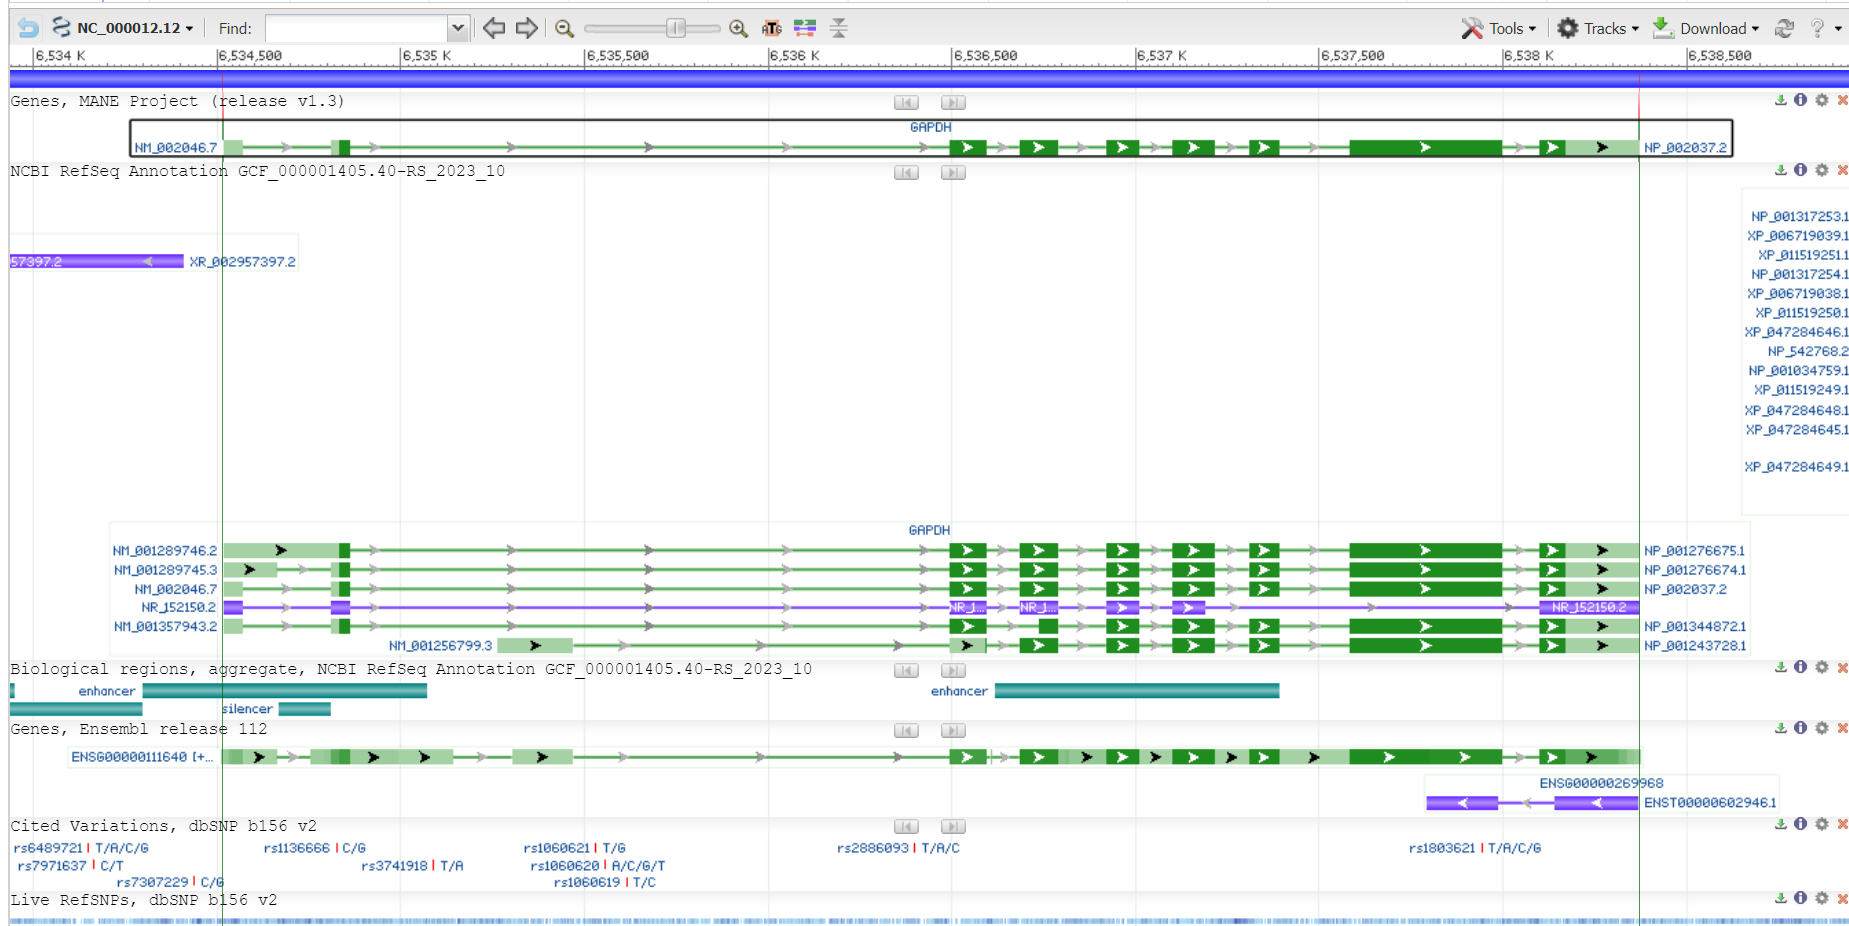
\includegraphics[width=\textwidth]{images/gapdh.png}
    \caption{Transkriptvarianten und Exons des GAPDH Gens \cite{NCBIGene2597_products}}
    \label{fig:exons}
\end{figure}

\subsection*{Spektroskopie zur Bestimmung der Nukleinsäurenkonzentration}

\begin{table}[H]
    \centering
    \begin{tabular}{lrrr}
    \toprule
    Sample name & Conc. (ng/uL) & 260/280[nm] & 260/230[nm] \\
    \midrule
    HEK293T & 115.449 & 2.098 & 2.069 \\
    HEK293T & 123.755 & 2.092 & 1.889 \\
    A375 & 442.625 & 2.119 & 2.164 \\
    A375 & 444.200 & 2.116 & 2.189 \\
    SAAA & 174.067 & 2.128 & 1.982 \\
    SAAA & 162.606 & 2.125 & 1.987 \\
    JEEE & 257.267 & 2.112 & 2.084 \\
    JEEE & 253.345 & 2.133 & 2.078 \\
    \bottomrule
    \end{tabular}
    \caption{Verhältnis der Absorption der Wellenlänge 260/280 [nm] und 260/230 [nm] der Proben}
\end{table}

Die Reinheit der RNA wird durch die 260/280- und 260/230-Verhältnisse bestimmt. Ein ideales 260/280-Verhältnis für RNA liegt bei etwa 2.0, was auf eine hohe Reinheit hinweist. Ein 260/230-Verhältnis sollte typischerweise zwischen 2.0 und 2.2 liegen, was auf das Fehlen von Verunreinigungen wie EDTA, Kohlenhydraten oder Phenolen hinweist \cite{ThermoFisher260280, ThermoFisherQuantitatingRNA}.

\textbf{Interpretation der Ergebnisse:}
\begin{figure}[H]
    \centering
    \begin{minipage}[H]{0.45\textwidth}
      \centering
      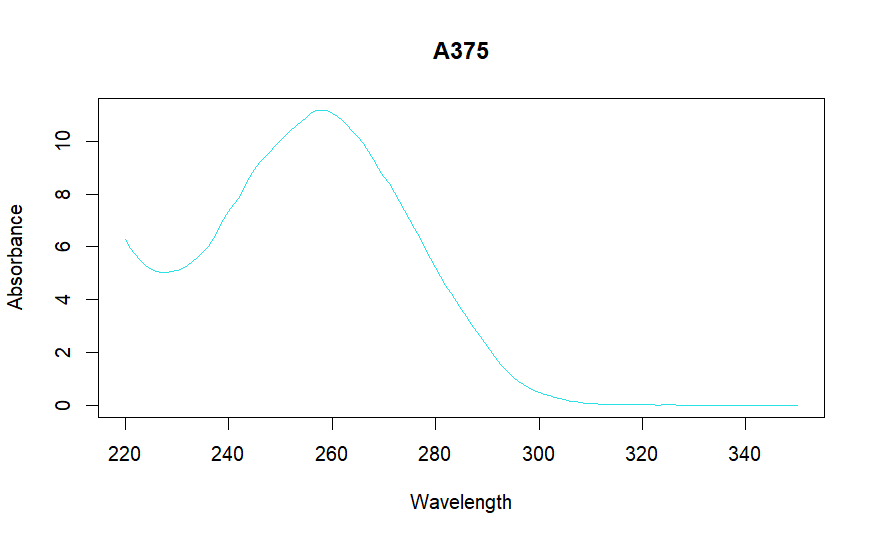
\includegraphics[width=\textwidth]{images/a3751.png}
      \caption{Absorptionsspektrum der A375-Proben}
      \label{fig:a3751}
    \end{minipage}
    \hfill
    \begin{minipage}[H]{0.45\textwidth}
      \centering
      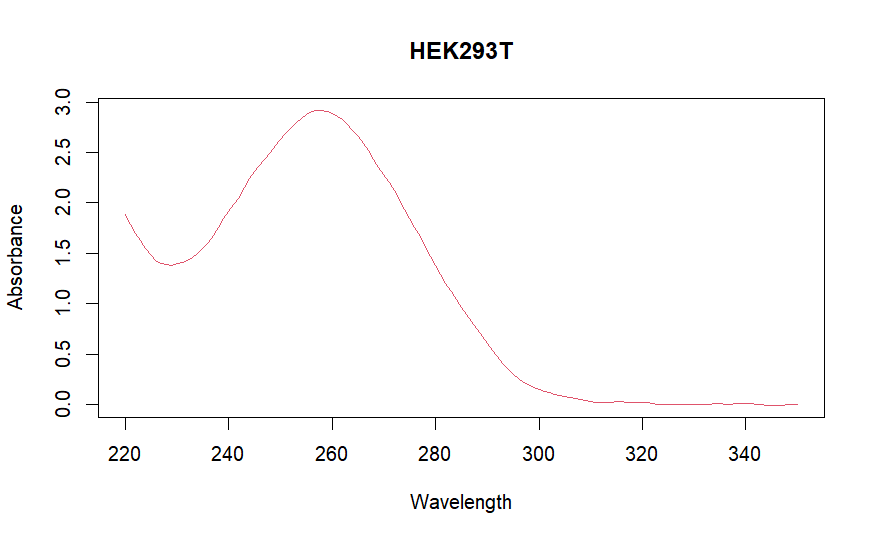
\includegraphics[width=\textwidth]{images/hek1.png}
      \caption{Absorptionsspektrum der HEK293T-Proben}
      \label{fig:hek1}
    \end{minipage}
  \end{figure}
\begin{itemize}
    \item \textbf{HEK293T}:
        \begin{itemize}
            \item Beide Proben zeigen ein 260/280-Verhältnis von etwa 2.09, was auf eine hohe Reinheit der RNA hinweist.
            \item Das 260/230-Verhältnis der ersten Probe (2.069) liegt im idealen Bereich, während das Verhältnis der zweiten Probe (1.889) leicht unter dem idealen Bereich liegt, was auf mögliche Kontaminationen hinweisen könnte.
        \end{itemize}

    \item \textbf{A375}:
        \begin{itemize}
            \item Beide Proben haben ein 260/280-Verhältnis von etwa 2.12, was eine gute RNA-Reinheit anzeigt.
            \item Das 260/230-Verhältnis liegt für beide Proben (2.164 und 2.189) im idealen Bereich, was auf eine sehr hohe Reinheit der RNA ohne signifikante Verunreinigungen hinweist.
        \end{itemize}
    
    \item \textbf{SAAA}:
        \begin{itemize}
            \item Beide Proben zeigen ein 260/280-Verhältnis von etwa 2.12, was auf eine hohe Reinheit hinweist.
            \item Die 260/230-Verhältnisse (1.982 und 1.987) sind leicht unter dem idealen Bereich, was auf geringe Verunreinigungen hindeuten könnte, jedoch immer noch akzeptabel ist.
        \end{itemize}
    \item \textbf{JEEE}:
        \begin{itemize}
            \item Beide Proben zeigen ein 260/280-Verhältnis von etwa 2.12 bis 2.13, was auf eine hohe Reinheit hinweist.
            \item Das 260/230-Verhältnis (2.084 und 2.078) liegt im idealen Bereich, was auf eine hohe Reinheit der RNA hinweist.
        \end{itemize}
\end{itemize}

Die meisten Proben zeigen 260/280- und 260/230-Verhältnisse, die nahe oder im idealen Bereich liegen, was auf eine hohe Reinheit der isolierten RNA hinweist. Einige leichte Abweichungen beim 260/230-Verhältnis könnten auf minimale Verunreinigungen hinweisen, die jedoch die Gesamtqualität der RNA nicht signifikant beeinträchtigen sollten.

\subsection*{PCR-Ergebnisse}

\begin{figure}[H]
    \centering
    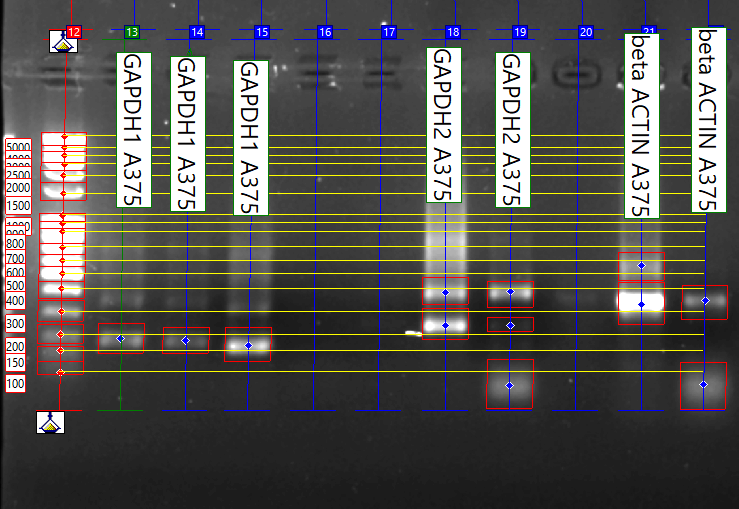
\includegraphics[width=\textwidth]{images/gel/a375bp.png}
    \caption{Agarose-Gel-Elektrophorese der PCR-Produkte der A375-Proben}
    \label{fig:gela375}
\end{figure}
\begin{figure}[H]
    \centering
    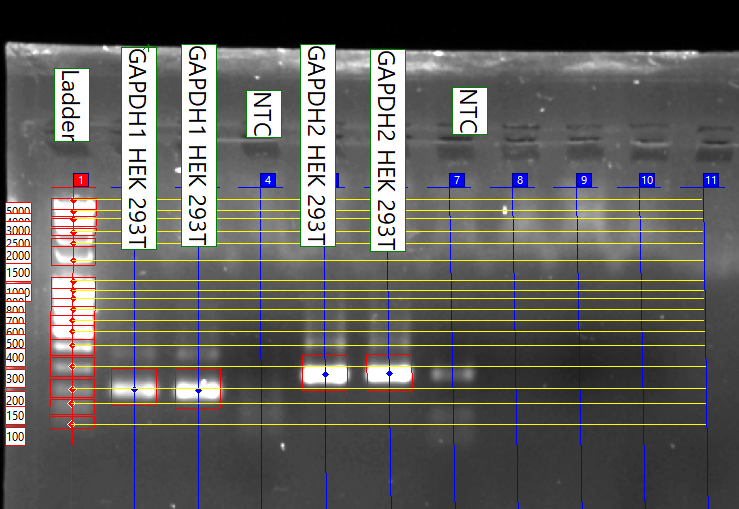
\includegraphics[width=\textwidth]{images/gel/hek293T.png}
    \caption{Agarose-Gel-Elektrophorese der PCR-Produkte der HEK293T-Proben}
    \label{fig:gela375}
\end{figure}

\subsection*{High Resolution Melting (HRM) Analyse}
\begin{figure}[H]
    \centering
    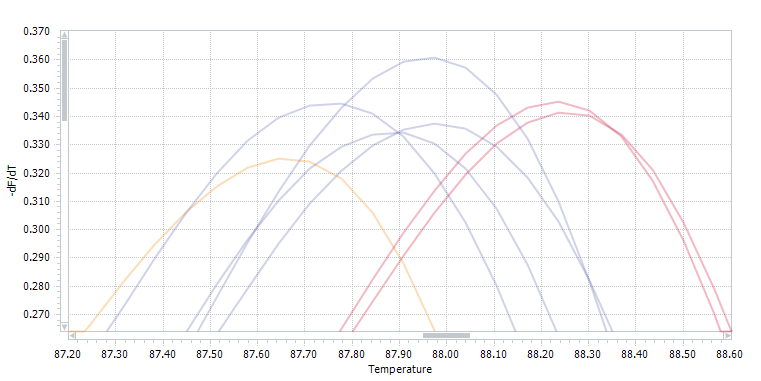
\includegraphics[width=\textwidth]{images/cycler/mc2.png}
    \caption{Schmelzkurven der GAPDH-Proben}
    \label{fig:gapdh}
\end{figure}
\subsection*{qPCR-Ergebnisse}
\begin{figure}[H]
    \centering
    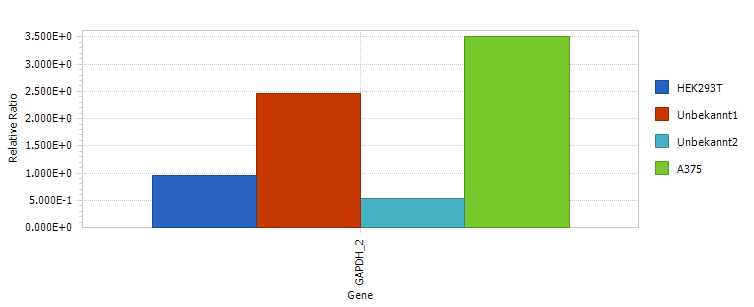
\includegraphics[width=\textwidth]{images/cycler/G1_2_G2.png}
    \caption{Verhältnisse der Amplifikationen der GAPDH-Proben}
    \label{fig:gapdh}
\end{figure}
\begin{figure}[H]
    \centering
    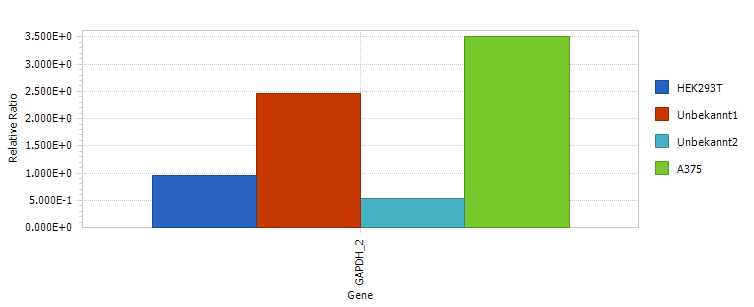
\includegraphics[width=\textwidth]{images/cycler/G1_2_G2.png}
    \caption{Verhältnisse der Amplifikationen der GAPDH-Proben zu Beta-Actin}
    \label{fig:gapdh2beta}
\end{figure}
% Diskussion
\section{Diskussion}



% Literaturverzeichnis
\bibliographystyle{plain}
\bibliography{references}

\end{document}
